\chapter{Design}
    This chapter is divided into multiple sections:
    \begin{itemize}
        \item We first explain what the components that collaborate with the oscilloscope are.
        \item We then provide extensions of $\Delta$QSD definitions, to fit the paradigm to work for our oscilloscope.
        \item Lastly, we explain the concept of triggers and snapshots, which make our $\Delta$Q oscilloscope comparable to a real one.
    \end{itemize}

    \section{Scenario}
    We can define four parts of interest for our tool.
    \paragraph{System under test} The system under test is the Erlang system the engineer wishes to observe, it ideally is a system which already is instrumented with OpenTelemetry. The ideal system where $\Delta$QSD is more useful is a system that executes many independent instances of the same action.
    
    \paragraph{Stub/wrapper} The stub is the \texttt{otel\_wrapper}, a wrapper that starts and ends OpenTelemetry spans, and start custom spans which are useful for the oscilloscope. Further handling of OpenTelemetry spans is delegated to the user, who may wish to do further operations with their spans. 
    The custom spans can be ended normally like OpenTelemetry spans or can timeout, given a custom timeout, and fail, according to user's definition of failure. \\
    The stub is called from the system under test and communicates spans data to the oscilloscope via TCP. \\
    The stub can receive messages from the oscilloscope, the messages are about updating observable's $dMax$.
    
    \paragraph{Server} The server is responsible for receiving the messages containing the custom spans from the oscilloscope. The server forwards the spans to the oscilloscope.
    
    \paragraph{Oscilloscope} The oscilloscope receives the custom spans from the stub and creates samples from said spans. \\
    The oscilloscope has a graphical interface which allows the user to create an outcome diagram of the system under test, display real time graphs which show detail about the execution of the system and allow the user to set custom timeouts for observables.

    \begin{figure}[H]
    \begin{center}
        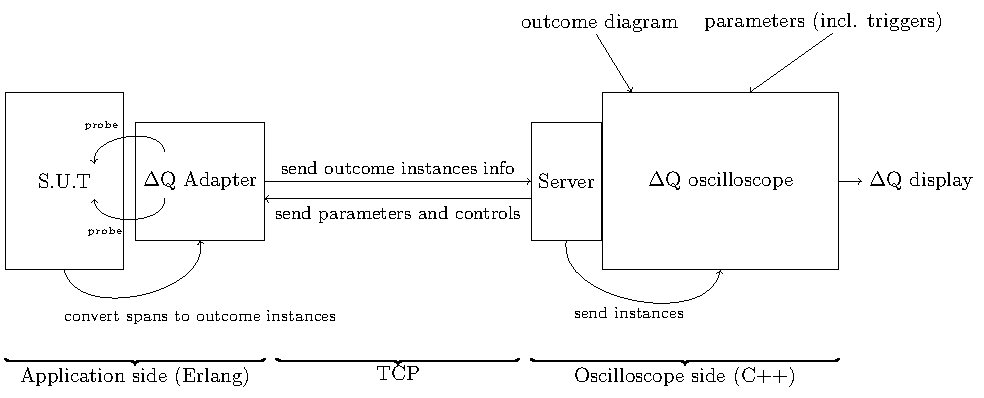
\includegraphics{tikz/sut-stub-osc.pdf}
    \end{center}
    \caption{Global system diagram: the SUT calls the wrapper when starting, ending and failing spans. The spans are received by the server which processes them and sends them to the oscilloscope. The server communicates with the stub to update informations about the system under test ($dMax$)}
    \end{figure}

    \section{Extending the notion of failure}
    Whilst previously we defined as "an input message $m_{in}$ that has no output message $m_{out}$", we extend this definition. If you recall the introduction \ref{timeout}, we introduced the notion of a maximum delay.

    We extend the notion of failure to the following definition:
        \begin{center}
            \textit{"An input message $m_{in}$ that has no output message $m_{out}$ after $x$ seconds"}
        \end{center}
    Where $x$ is the $dMax$ defined by the user. We can leverage this new definition to observe $\Delta$Qs in real time.


    \section{Time series - Oscilloscope outcome instances}
    Consider a probe $p$ with two distinct sets of events, the starting set of events $s$ and ending set of event $e$. The outcome instance of a message $m_s \rightarrow m_e$:
    \begin{itemize}
        \item The probe's $p$ name
        \item The start time $t_s$
        \item The end time $t_e$
        \item Its status 
        \item Its elapsed time of execution
    \end{itemize}
    The instance has three possible statuses: \texttt{success, timeout, failure}, it can thus be broken down in the representations, based on its status:
    \begin{itemize}
        \item \textbf{($t_s$,$t_e$)}: This representation indicates that the execution was successful (t $<$ $dMax$). 
        \item \textbf{($t_s, \mathcal{T}$)}: This representation indicates that the execution has timed out (t $>$ $dMax$). The end time and elapsed time is equal to $t_s + \text{timeout}$ 
        \item \textbf{($t_s, \mathcal{F}$)}: This representation indicates the execution has failed given a user defined requirement (i.e. a dropped message given buffer overload in a queue system). It must not be confused with a program failure (crash), if a program crashes during the execution of event $e$, it will time out since the wrapper will not receive an end message.
    \end{itemize}
    The \textbf{time series} of a probe is the sequence of $n$ outcome instances and can then be easily modeled by $\Delta$Q.

    \paragraph{What can be considered a failed execution?} Imagine a queue with a buffer: the buffer queue being full and dropping incoming messages can be modeled as a failure.

    More generally, the choice of what is considered a failed execution is left up to the user who is handling the spans and is program-dependent. Exceptions or errors can be kinds of failure. 

    On another note, the way of handling errored spans in OpenTelemetry can differ from user to user, so the wrapper will not handle ending and setting statuses for "failed" spans.
   

    \section{Probes}

To observe the system under test, the resulting outcomes, the result of causal links and outcome expressions, we must put probes in the system. \\
For each outcome of interest, a probe (observation point) is attached to measure the delay of the outcome, like one would in a true oscilloscope. \\
These probes allow to connect the system under test to the stub, which in turns sends a time series of data to the oscilloscope, which performs statistical computations on all the time series. \\
    Consider the figure below, a probe is attached at every component to measure the delay of N outcome ($p_2, p_3$), the stub will send the outcome instance data for each probe observing an outcome to the oscilloscope, which will measure their respective $\Delta$Qs from the time series data and display them (if chosen by the user). \\
    Another probe ($p_1$) is inserted at the beginning and end of the system to measure the global execution delay. \\
    Thanks to this probe, the user can observe the $\Delta$Q \textit{"observed at $p_1$"}, which is the $\Delta$Q which was calculated from the data received by inserting probe $p_1$. The \textit{$\Delta$Q "calculated at $p_1$"} is the resulting $\Delta$Q from the convolution of the observed $\Delta$Qs at $c_2$ and $c_3$.   
    \begin{figure}[H]
        \begin{center}
            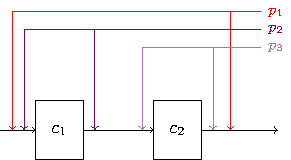
\includegraphics[scale=1.8]{tikz/probes.pdf}
        \end{center}
    \end{figure}

    \section{Triggers}
    Much like an oscilloscope that has a trigger mechanism to capture periodic signals or investigate a transient event \cite{osc-t}, the \textit{$\Delta$Q oscilloscope} has a similar mechanism that can recognise when an observed $\Delta$Q violates certain conditions regarding required behaviour and record snapshots of the system.

    Each time an observed $\Delta$Q is calculated, it is checked against the requirements set by the user. If these requirements are not met, a trigger is fired and a snapshot of the system is saved to be shown to the user. 
    
    \subsection{Snapshot}
    A snapshot of the system gives insights into the system before and after a trigger was fired. It gives the user a still of the system, as if it was frozen in time. All the $\Delta$Qs which are calculated during the system's execution are stored away. Then, if no trigger is fired, older $\Delta$Qs are removed. Otherwise, the oscilloscope keeps recording $\Delta$Qs without removing older ones, to allow the user to look at the state of the system before and after the trigger.
    

    \section{Polling window}
    To calculate a $\Delta$Q, we take all the outcome instances that ended within a window of time from $t_l$ to $t_u$, a lower and upper time bound.
    
    Suppose we are at time $t$, the window we will display is the  \textbf{window of time $(t-1)_{l}$ - $(t-1)_u$} with $t-1$ equal to $t - x$, and $x$ the polling rate. This is to account for various overheads that need to be taken into consideration, which could be network overhead, the wrapper overhead, C++ latency \dots Imagine multiple outcome instances that are ended at a time slightly lower but close to t, and due to the overheads the messages arrives at a time slightly higher but close to t, the outcome instance would not be taken into consideration for the calculation of a $\Delta$Q.
    
    \begin{figure}[H]
        \begin{center}
            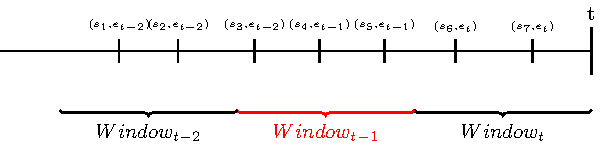
\includegraphics{tikz/window.pdf}
        \end{center}
    \end{figure}

    The polling window then advances every $x$ seconds setting the new window: 
    \begin{center}
        From: $(t-1)_l$, $(t-1)_u$ $\xrightarrow{t + 1}$ $t_l, t_u$. \\
        Where: $t_l = (t-1)_u$ and $t_u = (t-1)_u + x$ 
    \end{center}

